\section{From GMC to Pre-MS}

\subsection{Isothermal (approx) phase}

\begin{frame}{Jeans instability in isothermal pressure supported cloud}
\begin{columns}\begin{column}{0.5\textwidth}
\begin{itemize}
\item Jeans stability for molecular clouds: clouds not collapsing: thermal pressure/ interstellar magnetic field (large scale); \keyword{hydrostatic equilibrium for isothermal sphere}: (first approx for dense core/Bok globule: mechanical support from MHD waves diminish at this smaller scales)
\end{itemize}
\end{column}\begin{column}{0.5\textwidth}
\begin{align*}
&-\frac{1}{\rho}\nabla P-\nabla \phi=0\\
&P=\rho\frac{RT}{\mu}\\
&\nabla^2\phi=4\pi G\rho
\end{align*}
$\ln{\rho}+\phi/c_s^2$ spatial constant (spherical case):
\begin{equation*}
\rho(r)=\rho_c\Exp{-\phi/c_s^2}
\end{equation*}
\end{column}\end{columns}
\end{frame}

\begin{frame}{Isothermal Lane-Emden equation: \keyword{Gravitational stability using polytropes}}
\begin{columns}\begin{column}{0.5\textwidth}
\begin{align*}
&\frac{1}{r^2}\TDof{r}(r^2\TDy{r}{\phi})=4\pi G\rho=4\pi G\rho_c\exp{-\phi/c_s^2}\\
&\xi=\sqrt{\frac{4\pi G\rho_c}{c_s^2}}r,\ \psi=\frac{\phi}{c_s^2}\\
&\frac{1}{\xi^2}\TDof{\xi}(\xi^2\TDy{\xi}{\psi})=\exp{-\psi}\\
&M=4\pi\int_0^{r_0}\rho r^2\,dr=4\pi\rho_c(\frac{c_s^2}{4\pi G\rho_c})\expy{3/2}\int_0^{\xi_0}\exp{-\psi}\xi^2\,d\xi\\
&m=\frac{P_0\expy{1/2}G\expy{3/2}M}{c_s^4}=(4\pi\frac{\rho_c}{\rho_0})\expy{-1/2}(\xi^2\PDy{\xi}{\psi})_{\xi_0}
\end{align*}
\end{column}\begin{column}{0.5\textwidth}
\begin{figure}[!ht]
\centering
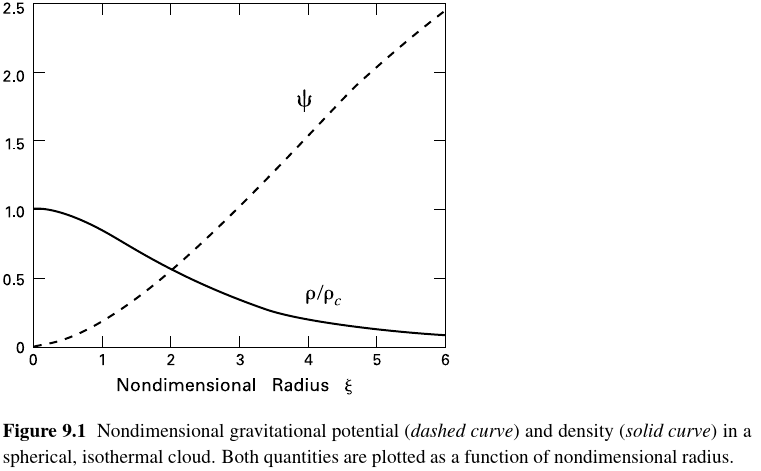
\includegraphics[trim={0cm 0cm 0 0},clip, keepaspectratio,width=0.99\textwidth]{polyadimprofile}
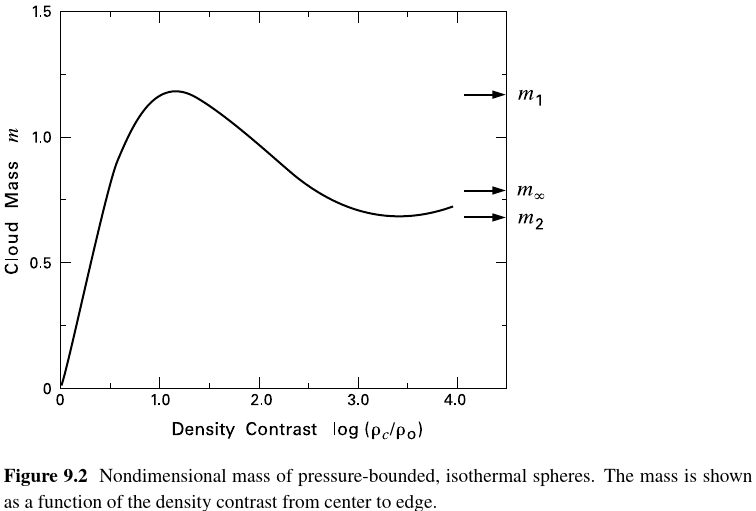
\includegraphics[trim={0cm 0 0 0},clip,width=0.99\textwidth]{polyadimmassvsdcontr}
\end{figure}
\end{column}\end{columns}
\begin{itemize}
\item Large distance $\xi\gg1$: $\frac{\rho}{\rho_c}\to\frac{2}{\xi^2}$
\end{itemize}
\end{frame}
 
\begin{wordonframe}{Radius as function of external pressure}
For small $\xi$ $\psi(\xi)\approx\frac{\xi^2}{6}+O(\xi^4)$:
\begin{equation*}
\frac{\rho_c}{\rho_0}=\exp{-\psi}\approx1-\frac{\xi_0^2}{6}
\end{equation*}
con $\rho_x/\rho_0\approx1$ si ha $r_0^3\approx\frac{3Mc_s^2}{4\pi P_0}$
\end{wordonframe}

\begin{frame}{Gravitational instability of iso-poly. Bonnor-Ebert mass}
All clouds with $\rho_c/\rho_0>14.1$ are gravitationally unstable those to the right of first maximum $M_{BE}=\frac{m_1c_s^4}{P_0\expy{1/2}G\expy{3/2}}$
\begin{figure}[!ht]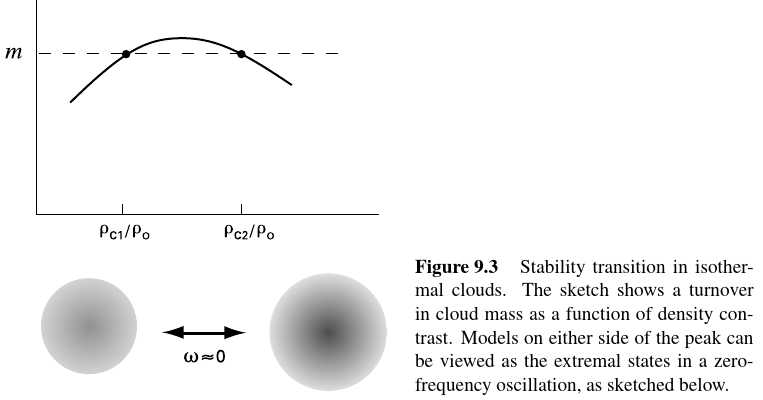
\includegraphics[trim={0cm 0cm 0 0},clip, keepaspectratio,height=0.5\textheight]{Gstabilityisopoly}\label{fig:Gstabilityisopoly}\end{figure}
\end{frame}

\begin{frame}{Jeans stability. Critical length scale}
Traveling(standing) waves solution stisfying momentum equation
\begin{align*}
&\rho\TDy{t}{\vec{u}}=-\nabla P-\rho\nabla\phi\\
&\rho(x,t)=\rho_0+\delta\rho\exp{i(kx-\omega t)}\ (\rho(x,t)=\rho_0(r)+\delta\rho(r)\exp{i\omega t})\\
&\omega^2=k^2c_s^2-4\pi G\rho_0
\end{align*}
\end{frame}

\begin{frame}{Stability for rotating clouds}
$\beta=\frac{\Omega_0^2R_0^3}{3GM}$: $\beta=1/3$ corrspond to break-up speed
\begin{figure}[!ht]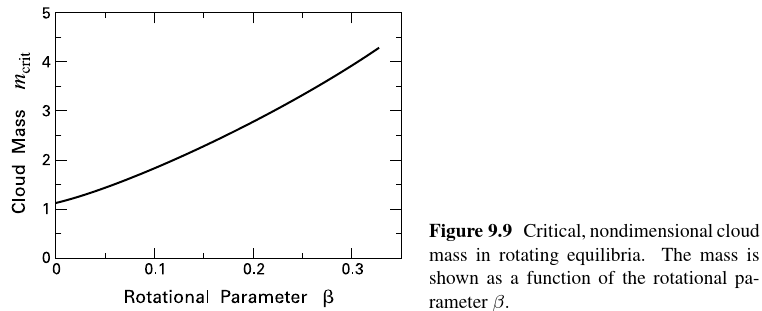
\includegraphics[trim={0cm 0cm 0 0},clip, keepaspectratio,width=0.4\textwidth]{mcritvsbetaclouds}\label{fig:mcritvsbetaclouds}\end{figure}
\end{frame}

\begin{wordonframe}{hydro-eq with rotational potential}
\begin{columns}[T]\begin{column}{0.5\textwidth}
\begin{align*}
&\varpi=r\sin{\theta}\\
&P=c_s^2\rho\\
&j=\varpi u_{\phi}\\
&\phi_{cen}=-\int_0^{\varpi}\frac{j^2}{\varpi^3}\,d\varpi
\end{align*}
\end{column}\begin{column}{0.5\textwidth}
\begin{align*}
&-\frac{c_s^2}{\rho}\nabla\rho-\nabla\phi-\nabla\phi_{cen}=0\\
&\rho(\vec{r})=\rho_c\exp{\frac{-\phi-\phi_{cen}-\phi(0)}{c_s^2}}
\end{align*}
\end{column}\end{columns}
\end{wordonframe}

\begin{frame}{Clouds fragmentation}

\end{frame}

\begin{frame}{Effects of magnetic field}
Palla stahler ch 9-10
\end{frame}

\subsection{Adiabatic phase}

%Inner region of collapsing cloud becomes denser/optically thicker: $df$

\section{GMC: turbolenza e campi magnetici}\linkdest{turbmagn}

\begin{wordonframe}{refx}
Theory of Star Formation - Mckee, Ostriker 07
\end{wordonframe}

\subsection{Kolmogorov theory}

\begin{frame}{Spatial correlation of velocity and magnetic field}
\begin{block}{autocorrelation function, structure function and power spectra}
$S_p(\vec{r})=\exv{|\vec{v}(\vec{x})-\vec{v}(\vec{x})|^p}$: RMS velocity difference is $\Delta v(\vec{r})=\sqrt{S_2(\vec{r})}$, autocorrelation is $A(\vec{r})=\exv{\vec{v}(\vec{x})\cdot\vec{v}(\vec{x}+\vec{r})}$;  lo spettro di potenza \'e FT di $A(\vec{r})$: $P(\vec{k})=|\vec{v}(\vec{k})|^2$, for zero mean velocity the velocity dispersion averaged over volume $l^3$ is $\sigma_v(l)^2=\int_{k_{min}}^{\infty}P(\vec{k})$ with $k_{min}=2\pi/l$
\end{block}
\begin{block}{Structure function, correlation function and power spectra}
magnetic field, and other fluid variables.
\end{block}
\end{frame}

\begin{frame}{Kolmogorov turbulence}
\begin{block}{Isotropy: $\vec{r}\to r$, $\vec{k}\to k$, $\vec{v}(\vec{k})\to v(l)=\delta v(l)$}
\begin{columns}[T]\begin{column}{0.5\textwidth}
$P(k)\propto k\expy{-n}$ (3D), $n'=n-2$ (1D angle-averaged)
\end{column}\begin{column}{0.5\textwidth}
$v(l)\propto\sigma_v(l)\propto\Delta  v(l)\propto l^q$, $q=(n-3)/2$
\end{column}\end{columns}
1D velocity dispersion along LOS is related to 3D velocity dispersion: $\sigma=\sigma_v(l)/\sqrt{3}$.
\end{block}
\end{frame}

\begin{frame}{Kolmogorov theory}
\begin{columns}[T]\begin{column}{0.5\textwidth}
\begin{block}{Incompressible flow}
$\sigma_v\ll\sigma_{th}=(P_{th}/\rho)\expy{1/2}$
\end{block}
\end{column}\begin{column}{0.5\textwidth}
\begin{block}{Raynold scale}
Energy is dissipated and turbulent motions are damped for scales smaller than Reynolds scale $l_{\nu}$: viscous term $\approx\nu v(l)/l^2$ exceeds nonlinear coupling terms between scales $v(l)^2/l$
\end{block}
\begin{block}{Rate energy transfer between scales}
larger than $l_{\nu}$, smaller than system scale: specific energy transfer
\[\dot{\mathcal{E}}\approx v(l)^3/l\Rightarrow n=11/3\]
\[S_3(l)=-4/5\dot{\mathcal{E}}l\]
\end{block}
\end{column}\end{columns}
\end{frame}

\begin{frame}{Turbulence in molecular clouds}
\[v(l)\propto\sigma_v(l)\propto\Delta  v(l)\lesssim c_s\]
some portion of energy is dissipated via shock: velocity discontinuity (1D) $P(k)\propto k\expy{-2}$, (3D) $n=4$
\begin{block}{Strong B}
$v_A=B/\sqrt{4\pi\rho}\gg v(l)$correlation of flow variables may depend differently on $\vec{r}_{\parallel}$, $\vec{r}_{\perp}$, $\vec{k}_{\parallel}$, $\vec{k}_{\perp}$
\end{block}
\begin{block}{Dissipation timescale}
Specific energy dissipation rate $\dot{\mathcal{E}}=\epsilon U^3/l_0$, $E=U^2/2$ total specific kinetic energy, $l_0$ spatial wavelenght of main energy containing scale; in GMC $l_0\to d$ diametro cloud, assumin g on average $U=\sigma_{los}\sqrt{3}$, flow crossing-time over main energy containing scale $t_f=l_0/U$ definisco turbulent dissipation timescale $\frac{E_{turb}}{|\dot{E}_{turb}|}=\frac{t_f}{2\epsilon}\approx0.5\frac{d}{\sigma_{los}}$
\end{block}
\end{frame}

\begin{frame}{Physical scales in GMC}
classical incompressible turbulence: outer $l_0$ and inner Reynolds scale $l_{\nu}$. Assuming Kolmogorov scaling $v(l)=v(l_0)(\frac{l}{l_0})\expy{1/3}$ dissipation scale
\[\frac{l_{\nu}}{l_0}=[\frac{\nu}{l_0v(l_0)}]\expy{3/4}=Re\expy{-3/4}\]
Mean free path for particles collision $\nu=c_s\lambda_{mfp}$:
\[\frac{l_{\nu}}{l_0}\approx(\frac{\lambda_{mfp}}{l_0})\expy{3/4}[\frac{v(l_0)}{c_s}]\expy{-3/4}\]
q closer to $1/2$ on large scale than $1/3$: supersonic compressible turbulence.
If $v(l_s)=c_s$: $\lambda_{mfp}\approx\SI{e13}{\cm}$, $l_s\approx\SI{0.03}{\parsec}$, $l_{\nu}\approx\SI{3e-5}{\parsec}$: density perturbation in non magnetic GMC with characteristic lenght $l_s$ will have order unity amplitude.
Flow along magnitic field will be as for unmagnetized medium, flow orthogonal to magnetic field will create order-unity density perturbation if  $v>\sqrt{c_s^2+v^2}$.
\end{frame}

\begin{frame}{Physical scales in GMC: with magnetic field}
MHD turbulence in fully ionized gas: below resistive scale Ohmic diffusion smooth out strong bends in magnetic field, allows folded lines to reconnect: magnetic induction equation, diffusion term $\eta B(l)/(4\pi l^2)=v(l)B(l)/l$ flux dragging term.
Weakly ionized medium: ambipolar diffusion (ion-neutral drift) becomes important before resistive scale is reached - smallest scale at which magnetic field is well coupled to bulk of gas: ion-neutral drift speed $B_0\delta B(m_i+m)/(4\pi\rho_i\rho\alpha_{in}l)=\delta v\approx\delta B/(4\pi\rho)$ turbulent velocity, $\alpha_{in}=\exv{\sigma_{in}|v_i-v_n|}\approx\SI{2e-9}{\cubic\cm\per\second}$
\[l_{AD}=\frac{v_A}{n_i\alpha_{in}}\approx\SI{0.5}{\parsec}(\frac{v_A}{\SI{3}{\kilo\meter\per\second}})(\frac{n_i}{\SI{e-3}{\per\cubic\cm}})\expy{-1}\]
For $\lambda<\pi l_{AD}$ MHD waves are unable to propagate in couples neutral-ion fluid: collision frequency of neutral with ion $n_i\alpha_{in}$ is less then half the wave frequency $\omega=kv_A$, for $\lambda>\pi l_{AD}$ MHD waves are damped at rate $\omega\pi l_{AD}/\lambda$
\end{frame}

\section{Formazione stellare: stabilit\'a}\linkdest{stability}

\subsection{Fase isoterma}

\begin{frame}{Collasso nube inter-stellare}

\begin{block}{Condizione di collasso}
Prima fase: collasso isotermo.
\begin{columns}
\begin{column}{0.5\textwidth}
$\TtwoDy{t}{I}<0$ quindi $E_T+U<0$.
\end{column}
\begin{column}{0.5\textwidth}
Nube di $H_2$ a $T=\SI{10}{\kelvin}$:
$\rho>\num{e-18}(\frac{M}{\msun{}})^{-2}$\si{\gram\per\cubic\cm}
\end{column}
\end{columns}
\end{block}
\begin{block}{Nubi giganti: addensamenti}
Turbolenza crea zone pi\'u dense: Mckee ostriker 07, Folin i 14, bertelli Motta 16.
\end{block}
\begin{block}{Rotazione}
\begin{columns}[T]
\begin{column}{0.5\textwidth}
T,M,J costanti:
\begin{align*}
&E_{th}\approx c'\\
&E_{Rot}\approx c''\rho\expy{\frac{2}{3}}\\
&U\approx c'''\rho\expy{\frac{1}{3}}\\
&\alpha=\frac{E_{th}}{U},\ \beta=\frac{E_{rot}}{U}
\end{align*}
\end{column}
\begin{column}{0.5\textwidth}
Condizione di collasso proibito: $16\alpha(\rho_0)\beta(\rho_0))>1$
\end{column}
\end{columns}
\end{block}
\end{frame}

\begin{wordonframe}{Collasso nube inter-stellare}\tolbf
\begin{block}{Teorema viriale:todo}\end{block}
\begin{columns}[T]
\begin{column}{0.5\textwidth}
T,M,J costanti:
\begin{align*}
&E_{th}\approx c'\\
&E_{Rot}\approx\frac{1}{2}\frac{J^2}{I}=\frac{J^2}{2}\frac{1}{\frac{2}{5}MR^2}=c''\rho\expy{\frac{2}{3}}\\
&U\approx\frac{3}{5}\frac{GM^2}{R}=c'''\rho\expy{\frac{1}{3}}
\end{align*}
\end{column}
\begin{column}{0.5\textwidth}
\begin{align*}
&f(\psi=\frac{\rho}{\rho_0})=\alpha_0\psi\expy{-\frac{1}{3}}+\beta_0\psi\expy{\frac{1}{3}}\\
&\begin{pmatrix}
&f<\frac{1}{2}: \text{collasso}\\
&f>\frac{1}{2}: \text{espansione}\\
\end{pmatrix}\\
&\alpha=\alpha_0(\rho_0)(\frac{\rho}{\rho_0})\expy{-\frac{1}{3}}\\
&\beta=\beta(\rho_0)(\frac{\rho}{\rho_0})\expy{\frac{1}{3}}
\end{align*}
\end{column}
\end{columns}
f ha minimo in $\psi_0=(\frac{\alpha_0}{\beta_0\beta_0})\expy{\frac{3}{2}}$
\end{wordonframe}

\subsection{Fase adiabatica}

\begin{frame}{Inizio fase adiabatica: aumento temperatura}
\begin{block}{Aumento cammino ottico}
\begin{columns}[T]
\begin{column}{0.5\textwidth}
Cammino ottico di un fotone minore delle dimensioni della nube: $\kappa\rho R>1$.
\end{column}
\begin{column}{0.5\textwidth}
Densit\'a che consente aumento T: $\rho_{ad}\propto M\expy{-\frac{1}{3}}?$
\end{column}
\end{columns}
\end{block}
\begin{block}{Termine collasso adiabatico ($\Delta E_T=-\Delta U$)}
Equilibrio: $E_T^{ad}+\Delta E_T=\frac{1}{2}|U+\Delta U|$: $\Delta R=-\frac{R}{2}$ e $\rho'=8\rho_{ad}$.
\end{block}
\begin{block}{Comportamento pseudo-adiabatico: $P\propto\rho\expy{\gamma}$}
\begin{columns}[T]
\begin{column}{0.5\textwidth}
\begin{align*}
&T=T_0(\frac{\rho}{\rho_{ad}})\expy{\gamma-1}\\
&P=P_0(\frac{\rho}{\rho_{ad}})\expy{\gamma}
\end{align*}
\end{column}
\begin{column}{0.5\textwidth}
$\gamma>\frac{4}{3}$: $\alpha$ diventa $>\frac{1}{2}$
\end{column}
\end{columns}
Condizione di equilibrio: $\rho_{eq}\propto M\expy{\theta}\begin{pmatrix}
\approx\num{e-10}, \gamma=\frac{5}{3}\\
\approx\num{e6}, \gamma=\frac{7}{5}
\end{pmatrix}$.
\end{block}
$T>\SI{e3}{\kelvin}$: dissociazione molecolare, ionizzazione.
Zona centrale raggiunge stato di quasi-equilibrio: lenta contrazione.
\end{frame}

\begin{wordonframe}{Fase adiabatica}
$P\propto\rho\expy{\gamma}$: corrisponde a vera adiabatica  se condizione iniziale di equilibrio o qe.

Condizione di equilibrio: $kT_0(\frac{\rho_{eq}}{\rho_{ad}})\expy{\gamma-1}=\const M\expy{\frac{2}{3}}\rho_{eq}\expy{\frac{1}{3}}$.

''Solo se la temperatura aumenta rapidamente con densit\'a \'e possibile ristabilire equilibrio.''

Ionizzazione e dissociazione rallentano aumento di T e P: accelerazione collasso.

Quando la zona interna raggiunge l'equilibrio l'esterno continua a contrarsi: rimbalzi.

\end{wordonframe}

\section{T tauri stars: young optically visible stars $M_*\leq2\msun$ (palla stealher 635)}

\begin{frame}{T-Tauri main chars}
\begin{columns}\begin{column}{0.5\textwidth}
\begin{itemize}
\item Proximity to molecular clouds
\item Youth: excess emission - photospheric radiation beyond that found in MS stars of same $T_e$
\end{itemize}
\end{column}\begin{column}{0.5\textwidth}

\end{column}\end{columns}

\end{frame}

